\chapter{Context} % Main chapter title
\label{chap:Context}

The concepts that were described in section \ref{sec:introduction_context} are essential for the correct understanding and analysis of the problem. For that reason, this chapter will present a deeper investigation on the concepts that are inherent to the business domain.
\par
Despite this project not being about retail of goods, it is still, in fact, a project about e-commerce, since it involves a commercial trade. The start of the chapter will start by introducing what is the E-Commerce Industry and explaining how e-commerce can be applied to services.

\section{E-Commerce Industry}
\label{sec:ecomIndustry}
By definition, "e-commerce refers to the use of electronic means and technologies to conduct commerce (sale, purchase, transfer or exchange of products, services and/or information" \parencite{introductionToECommerce}. This concept is as considered as old as internet itself. However, since internet was only for military use until 1991 \parencite{internetHistory}, the commercial activity wasn't very present until that time. 
\par
Amazon was one of the first online stores. Launched in 1995, this website was initially focused just on book selling. However, Jeff Bezos (Amazon's CEO) knew from the beginning that Amazon had to be "an everything store" \parencite{amazonHistory}. This vision propagated to other entrepreneurs, and after Amazon, many other competitors, like eBay (1995) and Alibaba (1999) appeared on the market. 
\par
The number of worldwide e-commerce sales has been increasing consistently and it is expected to continue this trend for the next years. The Figure  \ref{fig:ecommerceGrowth} shows how this trend has been for the last years and how it is predicted to be in the next few years.\footnote{data retrieved from https://www.statista.com/statistics/379046/worldwide-retail-e-commerce-sales/}

\begin{figure}[ht]
\centering
 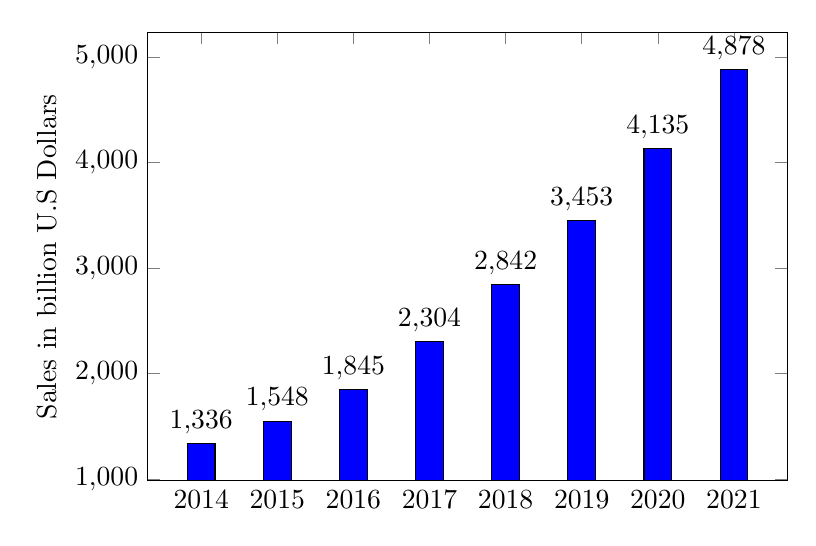
\begin{tikzpicture}
        \begin{axis}[
            symbolic x coords={2014, 2015, 2016, 2017, 2018, 2019, 2020, 2021},
            ylabel=Sales in billion U.S Dollars,
            width=0.8\textwidth,
            height=0.6\textwidth,
            nodes near coords,
            nodes near coords align={vertical},
          ]
            \addplot[ybar,fill=blue] coordinates {
                (2014,  1336)
                (2015,  1548)
                (2016,  1845)
                (2017,  2304)
                (2018,  2842)
                (2019,  3453)
                (2020,  4135)
                (2021,  4878)
            };
        \end{axis}
    \end{tikzpicture}
\caption{Worldwide e-commerce sales growth from 2014 to 2021}
\label{fig:ecommerceGrowth}
\end{figure}

This behavior is result of two facts. Firstly, society is more trustful on technology and the fear of fraud is more reduced now due to the current legislation, certifications given to trusted online stores and because new web-oriented payment methods having risen. The second reason is the high market competition that exists nowadays. Unlike the 90s and the early years of the \nth{21} century, there are a lot of online stores, selling almost everything that a customer might need.
\par

Despite the existence of ever more online stores and e-commerce platforms, the great majority of these platforms are engaged in the trade of physical products.

\section{E-Commerce applied to services}
\label{sec:ecommerceAppliedToServices}
As was explained on section \ref{sec:ecomIndustry}, most of e-commerce is done for buying physical products. This is done in the so called "online stores". However, the sale of services is a more contained, niche, market within this industry. Most of the services that are sold online are typically also virtual. Examples of those services are web hosting, cloud services and email accounts. It is, nevertheless, also possible to order some services online, like ordering an insurance contract but the range of options that exist is much more restricted.